%compile with pdflatex on papeeria

\documentclass[a4paper,12pt]{article}
\usepackage{fancyhdr}
\usepackage{fancyheadings}
\usepackage[ngerman,german]{babel}
\usepackage{german}
\usepackage[utf8]{inputenc}
%\usepackage[latin1]{inputenc}
\usepackage[active]{srcltx}
%\usepackage{algorithm}
%\usepackage[noend]{algorithmic}
\usepackage{amsmath}
\usepackage{amssymb}
\usepackage{amsthm}
\usepackage{bbm}
\usepackage{enumerate}
\usepackage{graphicx}
\usepackage{ifthen}
\usepackage{listings}
\usepackage{enumitem}
%\usepackage{struktex}
\usepackage{hyperref}
%\usepackage{tikz}

\pagenumbering{gobble}

%%%%%%%%%%%%%%%%%%%%%%%%%%%%%%%%%%%%%%%%%%%%%%%%%%%%%%
%%%%%%%%%%%%%% EDIT THIS PART %%%%%%%%%%%%%%%%%%%%%%%%
%%%%%%%%%%%%%%%%%%%%%%%%%%%%%%%%%%%%%%%%%%%%%%%%%%%%%%
\newcommand{\Fach}{2. Stegreifaufgabe aus der Mathematik (A)}
\newcommand{\Name}{}
\newcommand{\datum}{}
\newcommand{\Matrikelnummer}{}
\newcommand{\Semester}{Q12/2}
\newcommand{\Uebungsblatt}{} %  <-- UPDATE ME
%%%%%%%%%%%%%%%%%%%%%%%%%%%%%%%%%%%%%%%%%%%%%%%%%%%%%%
%%%%%%%%%%%%%%%%%%%%%%%%%%%%%%%%%%%%%%%%%%%%%%%%%%%%%%

\setlength{\parindent}{0em}
\topmargin -1.0cm
\oddsidemargin 0cm
\evensidemargin 0cm
\setlength{\textheight}{9.2in}
\setlength{\textwidth}{6.0in}

%%%%%%%%%%%%%%%
%% Aufgaben-COMMAND
\newcommand{\Aufgabe}[1]{
  {
  \vspace*{0.5cm}
  \textsf{\textbf{Aufgabe #1}}
  \vspace*{0.2cm}
  
  }
}
%%%%%%%%%%%%%%
\hypersetup{
    pdftitle={\Fach{}: Übungsblatt \Uebungsblatt{}},
    pdfauthor={\Name},
    pdfborder={0 0 0}
}

\lstset{ %
language=java,
basicstyle=\footnotesize\tt,
showtabs=false,
tabsize=2,
captionpos=b,
breaklines=true,
extendedchars=true,
showstringspaces=false,
flexiblecolumns=true,
}

\title{Übungsblatt \Uebungsblatt{}}
\author{\Name{}}

\begin{document}
\thispagestyle{fancy}
\lhead{\sf \large \Fach{} \\ %\small \Name{} - \Matrikelnummer{}
}
\rhead{\sf \Semester{} \\  \datum{}}
\vspace*{0.2cm}
%\begin{center}
%%\LARGE \sf \textbf{Übungsblatt \Uebungsblatt{}}
%\end{center}
%\vspace*{0.2cm}

%%%%%%%%%%%%%%%%%%%%%%%%%%%%%%%%%%%%%%%%%%%%%%%%%%%%%%
%% Insert your solutions here %%%%%%%%%%%%%%%%%%%%%%%%
%%%%%%%%%%%%%%%%%%%%%%%%%%%%%%%%%%%%%%%%%%%%%%%%%%%%%%

  Name: \underline{\hspace{7cm}}
  \hfill
  Datum: \underline{\hspace{4cm}}

\vspace{1cm}

%\begin{tikzpicture}[scale=0.5]
%    % Draw a line at 30 degrees and of length 3
%    %\draw (0,0) -- (0:2.5cm);
%  \draw[black] (0,0) -- (0,6) -- (5,9) -- (10,6);
%  \draw[black] (5,9) -- (12,11) -- (14,10);
%  \draw[black] (0,0) -- (10,0) -- (10,6);
%  \draw[black,thin,dashed]  (0,8) -- (4,3);
%  \draw[black,thin,dashed]  (2,3) -- (2,5);
%  \draw[red,dashed] (0,0) -- (3,1.5) -- (8,1.5);
%  \draw[red] (4,0) -- (5,0.5) -- (6.5,0.5) -- (8,1.5);
%\end{tikzpicture}


\Aufgabe{1:}
Die Abbildung zeigt modellhaft einen Gebäudekomplex, der auf einer horizontalen Fläche steht. Die Dachfirste sind parallel zur Grundfläche.

\begin{figure}[h]
  \centerline{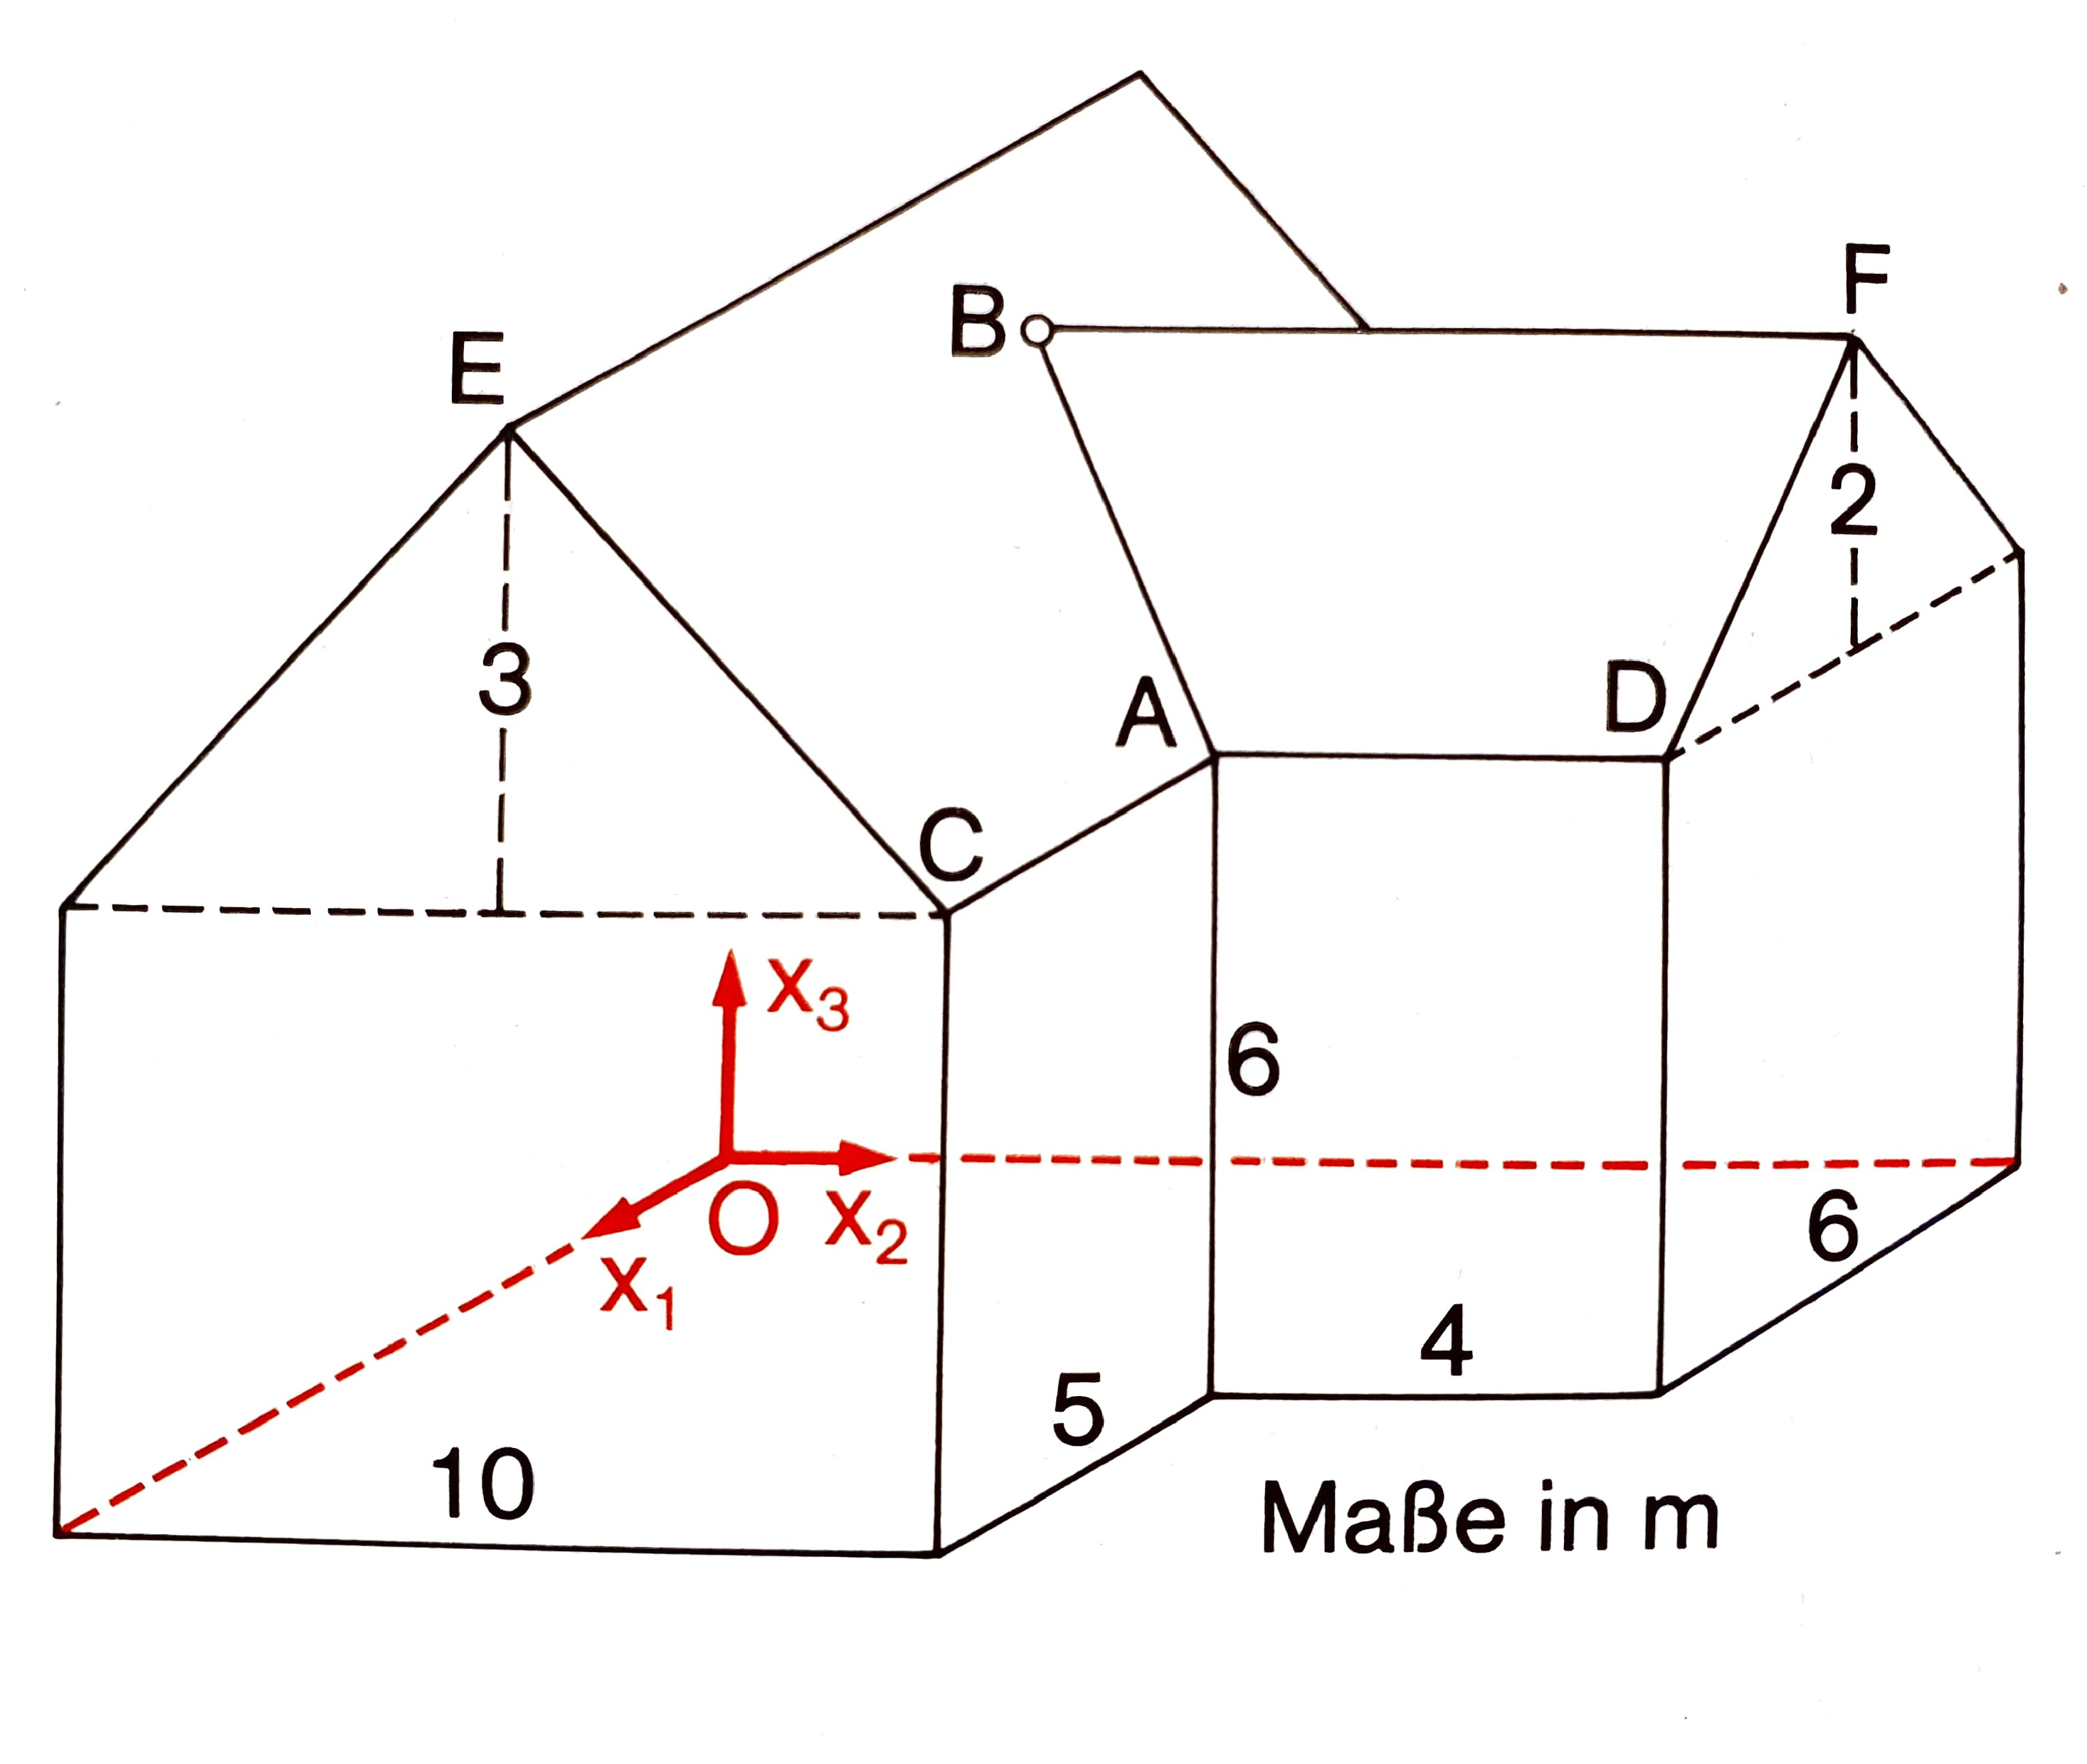
\includegraphics[scale=0.08]{hausBild.jpg}}
\end{figure}

\begin{enumerate}[label={\alph*)}]
\item Bestimmen Sie die Koordinaten von $A, C, D, E$ und $F$.
\begin{flushright}2,5 BE \end{flushright}
\item Berechnen Sie die Gleichung der Ebene $ACE$ in Normalenform.
\begin{flushright}4 BE \end{flushright}
\item Geben Sie die Gleichung der Geraden $BF$ an.
\begin{flushright}1,5 BE \end{flushright}
\item Berechnen Sie die Länge den Normalenvektor der Ebene $ACE$ und geben Sie die Hesse`sche Normalenform von $ACE$ in Vektor- und in Koordinatendarstellung an.
\end{enumerate}
\begin{flushright}3 BE \end{flushright}

  \vspace{1cm}
\begin{flushright}Bitte wenden $\Rightarrow$ \end{flushright}

\newpage
\Aufgabe{2:}
Untersuchen Sie jeweils die gegenseitige Lage der beiden Geraden $(\lambda;\mu \in \mathbb{R})$
\[
          g: \vec{X} = \begin{pmatrix}4 \\ 4 \\-1 \end{pmatrix} 
                     + \lambda \begin{pmatrix}1 \\ 2 \\2 \end{pmatrix}
            \quad
          h: \vec{X} = \begin{pmatrix}3 \\ 2 \\-3 \end{pmatrix}
                     + \mu \begin{pmatrix}2 \\ 0 \\2 \end{pmatrix}
\]

\begin{flushright}5BE \end{flushright}
\Aufgabe{3:}
Ermitteln Sie jeweils diejenigen Werte der Parameter $a$ und $b$, für die beiden Geraden
\[
  g: \vec{X} = \begin{pmatrix}6 \\ 0 \\ 0 \end{pmatrix} 
                     + \lambda \begin{pmatrix} a \\ -3 \\ 4 \end{pmatrix}
\quad \textrm{und} \quad
  h: \vec{X} = \begin{pmatrix}2 \\ 2 \\ b \end{pmatrix} 
                     + \mu \begin{pmatrix} 4 \\ -1,5 \\ 2 \end{pmatrix}
\]
echt parallel zueinander sind.\\
$
  (\lambda; \mu \in \mathbb{R})
$

\begin{flushright}4BE \end{flushright}



  \vspace{1cm}

\begin{center}Viel Erfolg! \end{center}







%%%%%%%%%%%%%%%%%%%%%%%%%%%%%%%%%%%%%%%%%%%%%%%%%%%%%%
%%%%%%%%%%%%%%%%%%%%%%%%%%%%%%%%%%%%%%%%%%%%%%%%%%%%%%
\end{document}
